% !TeX root = ../main.tex
% -*- coding: utf-8 -*-

\chapter{仿真实验与评估}

本文选择一种简单的民间纸牌游戏,来验证前面所提出的“自适应 Deep Q-Learning 算法”是否能够较为适应地处理现实中的实际问题。

\section{实验环境建立}

\subsection{纸牌游戏的背景与规则介绍}

在本游戏中,初始牌面会去掉 “红桃2”、“梅花2”、“方块2”、“黑桃A”这 4 张牌,共计 48 张牌,每人发牌 16 张。第一回合由持手牌“黑桃3”的玩家出牌,随后依逆时针顺序跟牌,且要求在能出牌的情况下必须出牌,不可直接过牌。

作为第一位玩家出牌时,可任意选择牌型出牌,而跟牌阶段则只能按规则在指定牌型下出牌,最先将手牌出完的玩家为胜者。

该游戏规则简单,共有以下几种牌型:

\begin{center}
    \tablecaption{牌型介绍}
\begin{tabular}{c|c|c|c}
    \toprule[2pt]
    {\jiacu\heiti 牌型简称} & {\jiacu\heiti 牌型描述} & {\jiacu\heiti 牌型简称} & {\jiacu\heiti 牌型描述} \\
    \midrule[2pt]
    对子 & 两张相同的牌 & 三条 & 三张相同的牌 \\
    % \hline
    炸弹 & 四张相同牌 & 三带一 & 三条+单牌 \\
    % \hline
    三带二 & 三条+任意两张牌 & 单顺 & 至少5张的连续牌 \\
    % \hline
    双顺 & 至少2组连续对子 & 三顺 & 至少2组连续三条 \\
    % \hline
    飞机 & 至少2组连续三带二 & 四带二 & 炸弹+任意两张牌\\
    \bottomrule[2pt]
\end{tabular}

\end{center}

\subsection{模拟建立的纸牌游戏环境}

基于游戏的基本规则,使用 \texttt{Python} 编程语言构建了一个简单的游戏模拟环境。为了能够进行数值化的模型训练,需要将不同纸牌转化为对应的数值编号,具体地,将游戏规则下一副牌(该规则下共 48 张牌)从 “黑桃3” 到 “方块2” 由小到大对应为一个长度为 48 的一维向量,每张牌都有一个唯一的 ID ,例如 \texttt{['黑桃3', '黑桃5', '红桃5', '梅花5', '黑桃7']} 转化后应为 \texttt{[0, 8, 9, 10, 16]}。后面的实验介绍中,模型内部结构均基于此前提。

在 \texttt{utils.py} 文件中,定义了 \texttt{divide\_cards()} 函数来实现发牌功能,能够随机将 48 张牌分为三份,发放给三位玩家,每位玩家各自分配到长度为 16 的一维向量,代表自己的手牌。

同时还定义了 \texttt{calculate\_score()} 函数,它能够根据游戏规则来计分,起到向模型传递反馈奖励值的作用。

在 \texttt{RunFastGame.py} 中,定义了一个完整的 \texttt{RunFastGameEnv} 类,它能够完整地模拟卡牌游戏对局,其中 \texttt{RunFastGameEnv.get\_state()} 函数能够获得当前所处的状态 $s$,\texttt{RunFastGameEnv.play\_cards()} 能够接收策略传入的指令来采取相应的行动 $a$。

具体地,\texttt{RunFastGameEnv} 能够模拟卡牌游戏对局中的每位玩家,它能基于环境信息以及模型的策略决策情况来模拟完整的游戏对局,从而产生了真实的经验数据,提供给模型进行 Monte Carlo 模拟,从而得以实现之前提出的算法。

\section{算法仿真与评估}

\subsection{Deep Q-Network 算法实现细节}

在 \texttt{DQN.py} 中,定义一个 \texttt{QNet} 类,建立一个全连接神经网络,其深度为 3 层。Input layer 有 209 个神经元,对应输入特征向量的 209 个元素;Hidden layer 1 有 512 个神经元;Hidden layer 2 有 256 个神经元;Hidden layer 3 有 128 个神经元;Output layer 只有一个神经元,其输出值为 $Q$ 函数所对应的值,如下图所示。

\begin{figure}[H]
    \centering
    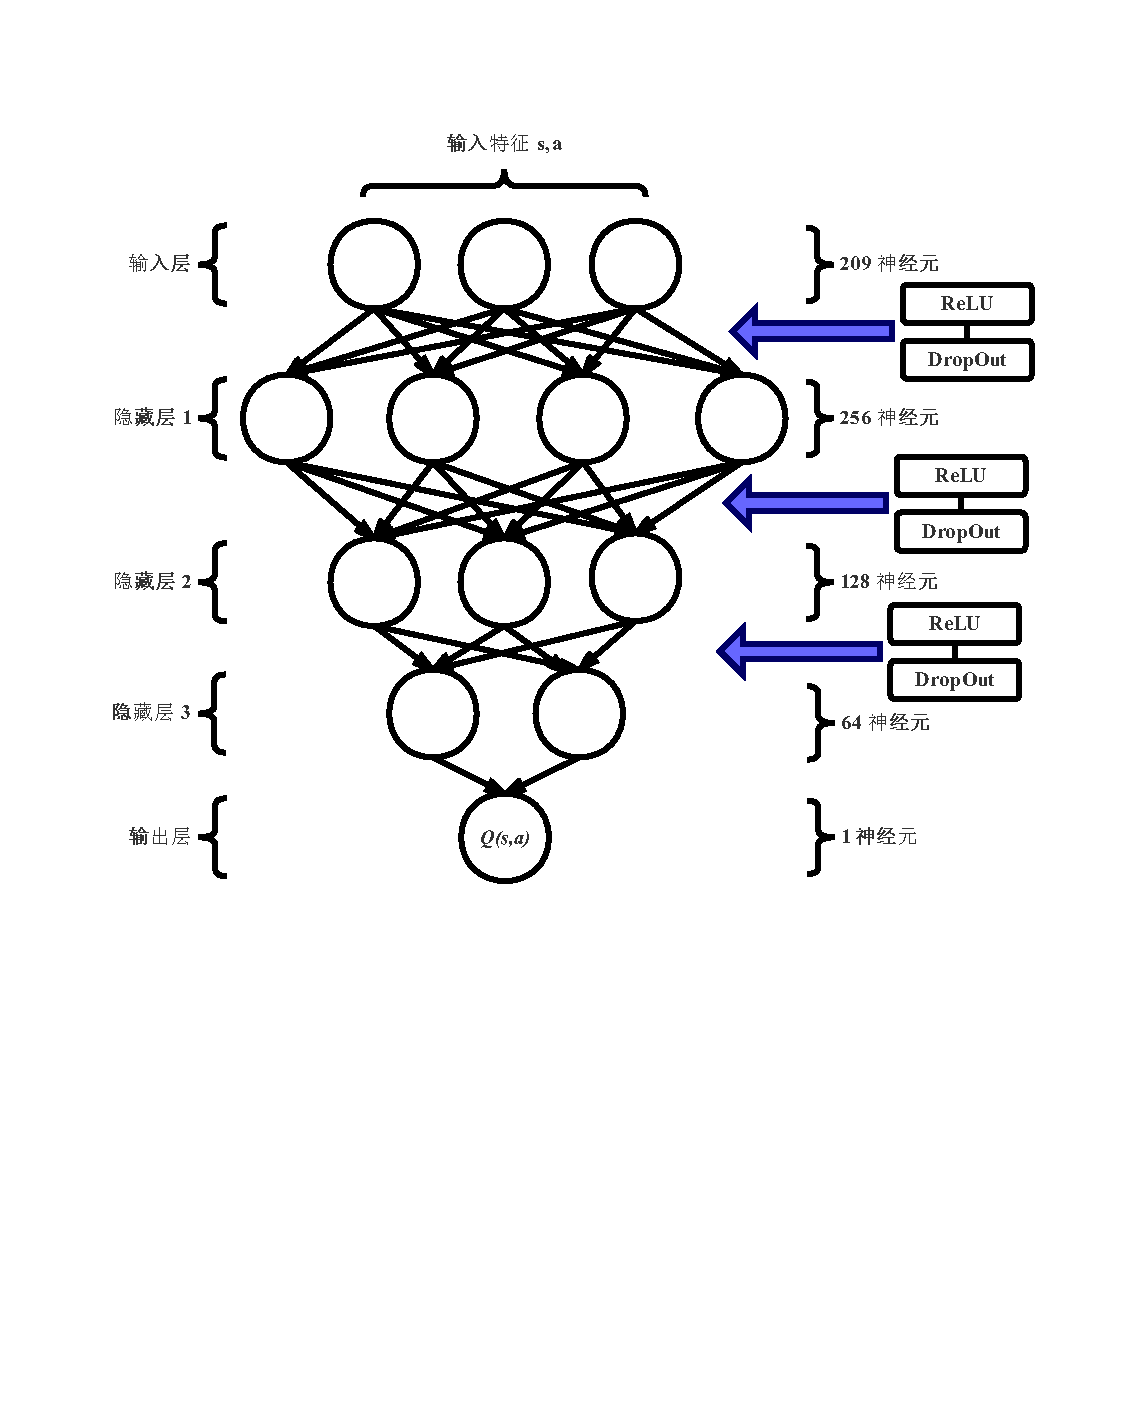
\includegraphics[width=0.8\textwidth]{DQN-Detail.pdf}
    \caption{Deep Q-Network 实现细节}
\end{figure}

此外还定义了一个 \texttt{DQN} 类,用来实现 Deep Q-Network 的细节。其中,\texttt{DQN.choose\_action()} 函数代表策略函数 $\pi$ ,其功能是根据输入的状态 $s$ ,根据 $Q$ 函数大小决定的策略概率分布 $\pi(a|s)$ 来决定下一步应采取的行动 $a$ ,其中

\begin{equation}
    \pi(a|s)=
    \begin{cases}
        \frac{\varepsilon}{|\mathcal A(s)|}&, a\neq\arg\max_aQ(s,a)\\
        1-\varepsilon-\frac{\varepsilon}{|\mathcal A(s)|}&, a=\arg\max_aQ(s,a)
    \end{cases}
\end{equation}

\texttt{DQN.store\_transition()} 函数和 \texttt{DQN.add\_reward()} 函数用于将模拟过程中的一些关键信息存储于缓存中;\texttt{DQN.learn()} 函数的作用是将缓存的信息提取出来,通过神经网络进行 Q-Learning 更新,更新公式为

\begin{equation}
    \widehat{Q}(S_t,A_t,\boldsymbol{w})\leftarrow \widehat{Q}(S_t,A_t,\boldsymbol{w})+\alpha\left[R_{t+1}+\gamma  \max\limits_a \widehat{Q}(S_{t+1},a,\boldsymbol{w})-\widehat{Q}(S_t,A_t,\boldsymbol{w})\right]
\end{equation}

最后,将 Deep Q-Network 模型接入进前面构建好的 \texttt{RunFastGameEnv} 环境下,即可开始模拟和训练的过程。

\subsection{仿真实验细节}

在前面所建立的仿真实验环境 \texttt{RunFastGameEnv} 中,由于是三人不完全信息博弈,即有 $N=3$,故总共需要建立六个 Deep Q-Network,每位玩家分配两个神经网络。

由于自适应 Deep Q-Learning 算法能够抵消估计偏差值,因此可以使用风格不同的三位玩家模型进行博弈训练,而风格差异化能够增加训练模型的鲁棒性,增强模型处理不确定性状态的能力。记三名玩家为分别为 $A,B,C$ ,其中 $A$ 玩家对应的模型为主训练模型,玩家 $B,C$ 为辅助学习模型,通过调整贪心率 $\varepsilon$ 使得辅助学习模型的决策水平与主训练模型形成差异化。其中 $\varepsilon_B = \frac{\varepsilon_A}{2}$ ,$\varepsilon_C = \frac{\varepsilon_A}{3}$。

此外,为了加速强化学习的学习效率,将算法中的贪心学习率 $\varepsilon$ 进行了动态调整,从初始值 $\varepsilon_0 = 0.4$ 随训练次数线性下降,每个 epoch 下降 0.01,达到预设的下限阈值 $\varepsilon_{stop} = 0.08$ 后停止动态调整。

基于前面所描述的细节,本实验的具体流程如下:

\begin{algorithm}[H]
    \caption{训练过程}
    \begin{algorithmic}[1] %每行不显示行号
        \State 初始化三名水平不同的玩家 $A, B, C$
        \Repeat
        \State 开始新一局游戏,并为三名玩家发牌
        \Repeat
        \State 根据游戏规则决定当前回合应当出牌的玩家
        \State 进入当前玩家的视角,根据场面信息获取当前所处状态 $S$
        \State 将状态 $S$ 传入 $Q$ 函数 和 $\pi$ 策略,决策下一步所要采取的行动 $a$
        \State 实际采取行动 $a$ ,接收环境传递的反馈值,并存入缓存
        \Until{执行行动 $a$ 后本局游戏分出胜负}
        \State 根据游戏规则,统计该局游戏各玩家得分,并追加存储至缓存
        \State 将缓存的信息,作为输入参数传入神经网络
        \State 经由神经网络完成一次训练学习,得到新的 $Q$ 函数和 $\pi$ 策略,用于下一次决策
        \Until{达到预设的训练次数}
        \State 结束训练,输出训练所得到的模型和参数
    \end{algorithmic}
\end{algorithm}

实验的流程图如下:

\begin{figure}[H]
    \centering
    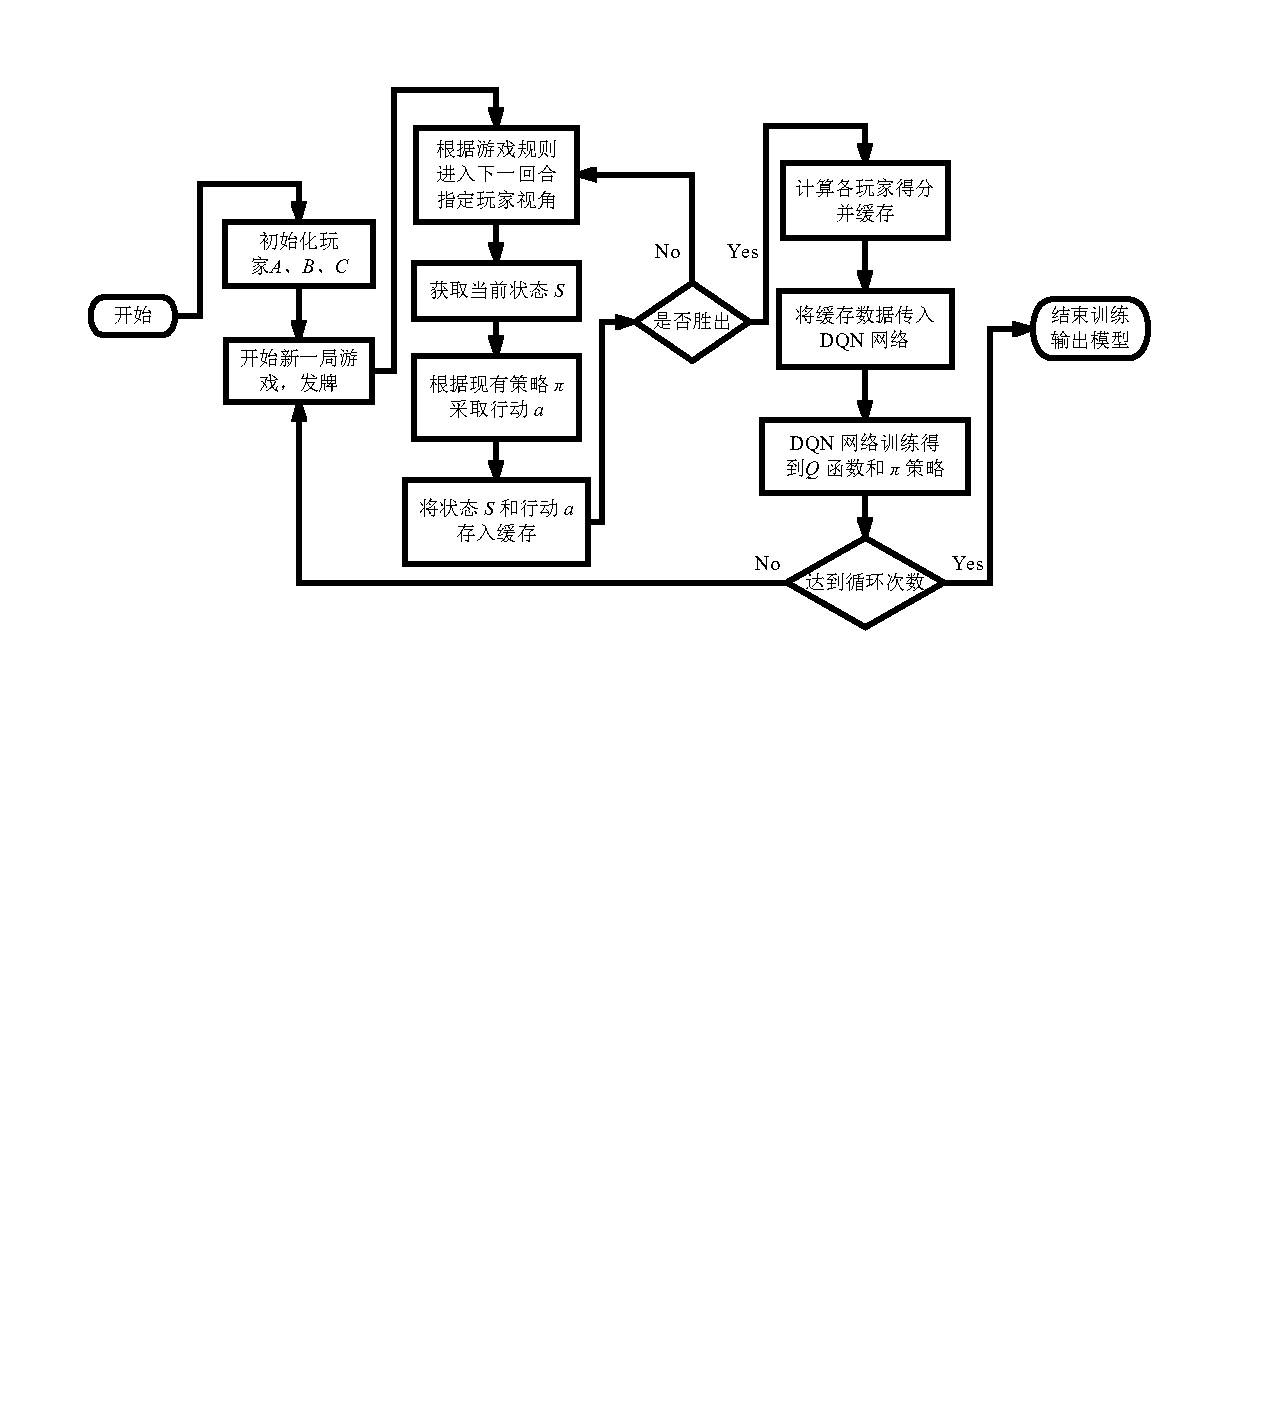
\includegraphics[width=\textwidth]{DQN-Process.pdf}
    \caption{实验流程图}
\end{figure}

\section{仿真实验结果与分析}

在 $\mathrm{NVIDIA}^\circledR$ GTX 1080 GPU 的硬件条件下,经过 50 万局自我对战学习(其中每 1000 局作为一个 epoch 集中学习),最终决策函数 $Q$ 得到如下图所示的收敛情况。

\begin{figure}[H]
	\centering
	\begin{subfigure}{0.45\textwidth} % width of left subfigure
		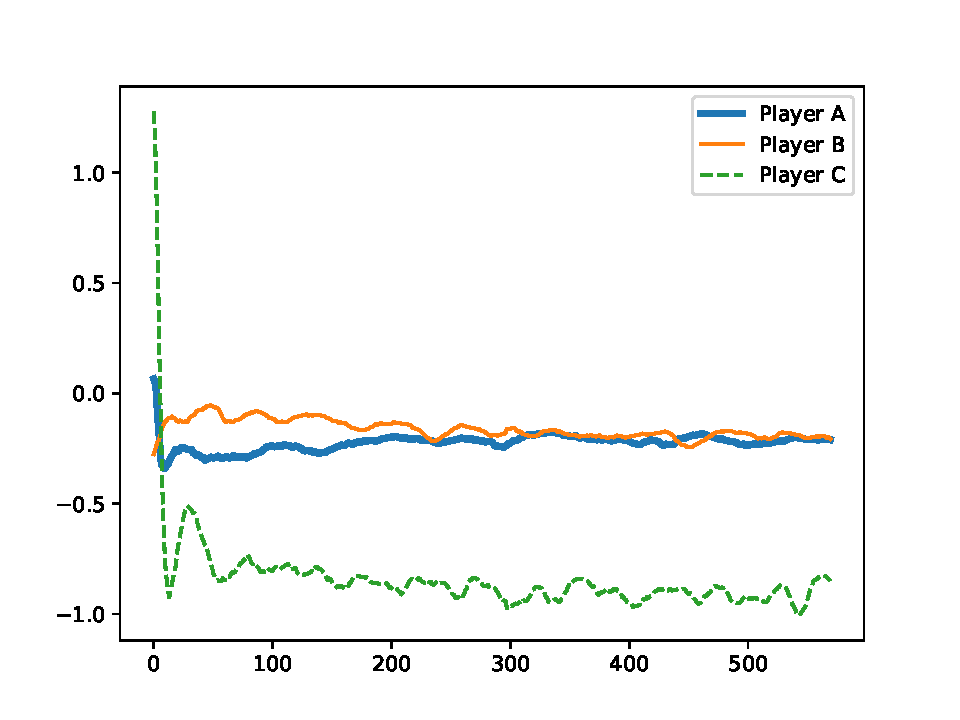
\includegraphics[width=\textwidth]{q-value.pdf}
		\caption{Q 函数训练均值}\label{img:q-value} % subcaption
	\end{subfigure}
	\vspace{1em} % here you can insert horizontal or vertical space
	\begin{subfigure}{0.45\textwidth} % width of right subfigure
		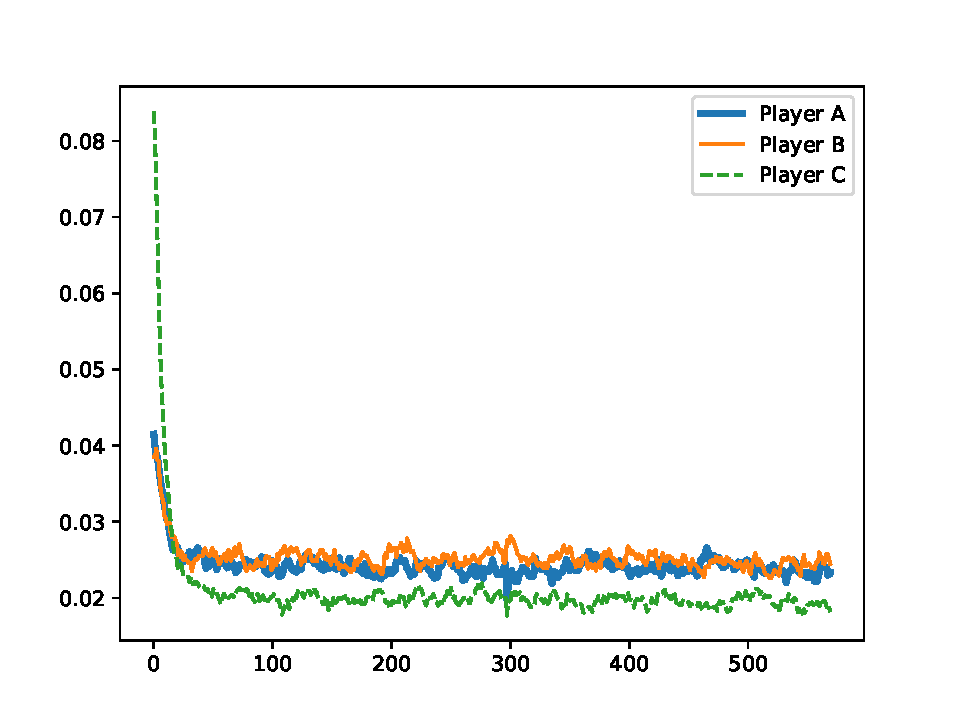
\includegraphics[width=\textwidth]{train-loss.pdf}
		\caption{Q-Learning 训练误差值}\label{img:train-loss} % subcaption
	\end{subfigure}
	\caption{仿真实验的训练结果} % caption for whole figure
\end{figure}

由图\ref{img:q-value},经过自适应 Deep Q-Learning 算法训练可使行动价值函数 $Q(s,a)$ 收敛,进而可以得到 $\varepsilon$-贪心策略:

\begin{equation}
    \pi(a|s)=
    \begin{cases}
        \frac{\varepsilon}{|\mathcal A(s)|}&, a\neq\arg\max_aQ(s,a)\\
        1-\varepsilon-\frac{\varepsilon}{|\mathcal A(s)|}&, a=\arg\max_aQ(s,a)
    \end{cases}
\end{equation}

其中策略 $\pi(a|s)$ 是一个条件概率分布,其含义是模型处于状态 $s$ 时,决定采取行动 $a$ 的概率。

另外,也可根据训练中的损失函数观察其收敛效果,图\ref{img:train-loss}所示的即为 自适应 Deep Q-Learning 算法的梯度损失项:

\begin{equation}
    \centering
    J(\boldsymbol{w}) = \frac{1}{2}\left[R_{t+1}+\gamma\max_a\widehat{Q}(S_{t+1},a,\boldsymbol{w})-\widehat{Q}(S_t,A_t,\boldsymbol{w})\right]^2
\end{equation}

从图中可观察知,损失项最后下降至一个较小值,Q 函数逐渐收敛。

\begin{figure}[H]
    \centering
    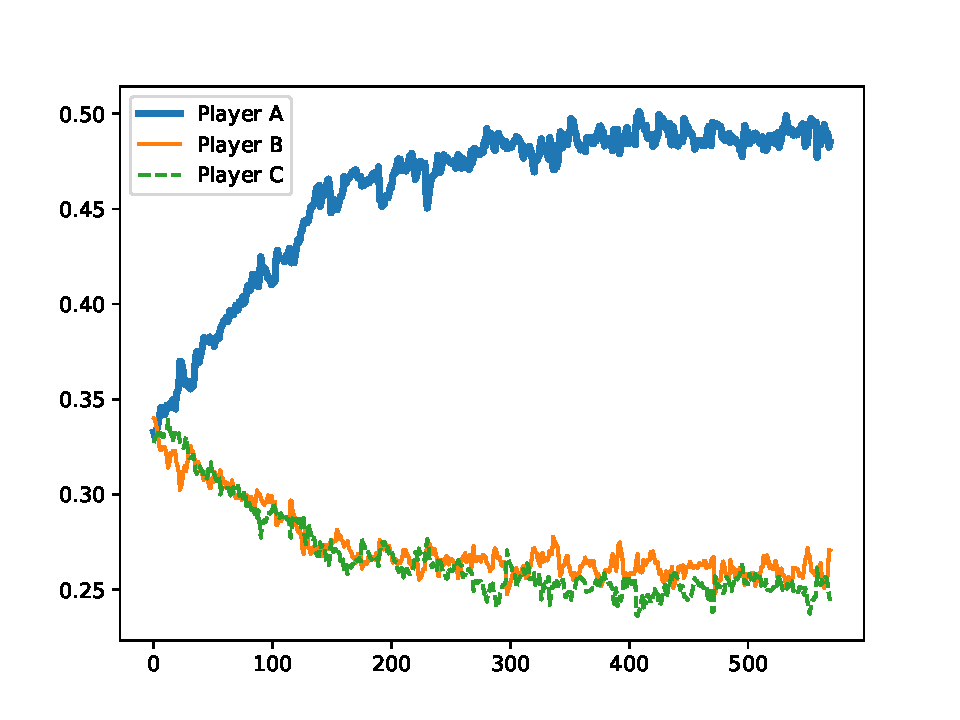
\includegraphics[width=0.8\textwidth]{win-rate.pdf}
    \caption{Q 函数与实时训练胜率}\label{img:win-rate}
\end{figure}

在训练中,还统计了三个玩家模型的实时胜率,如图\ref{img:win-rate}所示,可见在训练过程中,自适应 Deep Q-Learning 算法的主训练模型胜率不断上升,远优于另外两个辅助学习模型,显然自适应 Deep Q-Learning 算法通过强化学习的思想学习和掌握了一定程度的游戏技巧。

\begin{table}[H]
\caption{Multi-column table}
\begin{center}
\begin{tabular}{c|c|c|c|c|c}
    \toprule[2pt]
    \multicolumn{2}{c|}{主模型 A}&\multicolumn{2}{c}{辅助模型 B}&\multicolumn{2}{c}{辅助模型 C}\\
    % \hline
    $\varepsilon_A$&胜率&$\varepsilon_B$&胜率&$\varepsilon_C$&胜率\\
    \midrule[2pt]
    0.111&0.222&0.333&0.444&0.555&0.666\\
    % \hline
    0.111&0.222&0.333&0.444&0.555&0.666\\
    \bottomrule[2pt]
\end{tabular}
\end{center}
\label{tab:multicol}
\end{table}